% 
% Compile with 'pdflatex -shell-escape clojure-basics.tex'
% I use the mactex distro of Tex. https://tug.org/mactex/
% 

\documentclass{beamer}

\usetheme{Madrid}    

\usepackage{listings}                                   
\usepackage{hyperref}
\usepackage{graphicx}                                 
\usepackage{tabularx}
\usepackage{microtype}
\usepackage[T1]{fontenc}
\usepackage[scaled]{beramono}
\usepackage{minted}
\usepackage{xcolor}
\usepackage{pgfplots}
\usepackage{dirtytalk}
\usepackage{tikz}
\usetikzlibrary{tikzmark,fit}

%\usepackage{enumitem}
\pgfplotsset{compat=1.6} 

\newcommand\Small{\fontsize{5}{5.2}\selectfont}
\newcommand*\LSTfont{\Small\ttfamily\SetTracking{encoding=*}{-60}\lsstyle}
\renewcommand{\footnotesize}{\tiny}

\hypersetup{colorlinks=color, linkcolor=black}
\definecolor{OliveGreen}{rgb}{0,0.6,0}
\graphicspath{{./images/}}
% 
% Turn off beamer nav stuff...
% 
\setbeamertemplate{navigation symbols}{}


%
% listings does not currently support clojure...here's an attempt I
% found in a discussion thread to add clojure support.
% For the moment, this results in decent looking code. I might switch
% to minted in the future.
%
\lstdefinelanguage{clojure}%
{morekeywords={*,*1,*2,*3,*agent*,*allow-unresolved-vars*,*assert*,*clojure-version*,*command-line-args*,%
*compile-files*,*compile-path*,*e,*err*,*file*,*flush-on-newline*,*in*,*macro-meta*,%
*math-context*,*ns*,*out*,*print-dup*,*print-length*,*print-level*,*print-meta*,*print-readably*,%
*read-eval*,*source-path*,*use-context-classloader*,*warn-on-reflection*,+,-,->,->>,..,/,:else,%
<,<=,=,==,>,>=,@,accessor,aclone,add-classpath,add-watch,agent,agent-errors,aget,alength,alias,%
all-ns,alter,alter-meta!,alter-var-root,amap,ancestors,and,apply,areduce,array-map,aset,%
aset-boolean,aset-byte,aset-char,aset-double,aset-float,aset-int,aset-long,aset-short,assert,%
assoc,assoc!,assoc-in,associative?,atom,await,await-for,await1,bases,bean,bigdec,bigint,binding,%
bit-and,bit-and-not,bit-clear,bit-flip,bit-not,bit-or,bit-set,bit-shift-left,bit-shift-right,%
bit-test,bit-xor,boolean,boolean-array,booleans,bound-fn,bound-fn*,butlast,byte,byte-array,%
bytes,cast,char,char-array,char-escape-string,char-name-string,char?,chars,chunk,chunk-append,%
chunk-buffer,chunk-cons,chunk-first,chunk-next,chunk-rest,chunked-seq?,class,class?,%
clear-agent-errors,clojure-version,coll?,comment,commute,comp,comparator,compare,compare-and-set!,%
compile,complement,concat,cond,condp,conj,conj!,cons,constantly,construct-proxy,contains?,count,%
counted?,create-ns,create-struct,cycle,dec,decimal?,declare,def,definline,defmacro,defmethod,%
defmulti,defn,defn-,defonce,defprotocol,defstruct,deftype,delay,delay?,deliver,deref,derive,%
descendants,destructure,disj,disj!,dissoc,dissoc!,distinct,distinct?,do,do-template,doall,doc,%
dorun,doseq,dosync,dotimes,doto,double,double-array,doubles,drop,drop-last,drop-while,empty,empty?,%
ensure,enumeration-seq,eval,even?,every?,false,false?,ffirst,file-seq,filter,finally,find,find-doc,%
find-ns,find-var,first,float,float-array,float?,floats,flush,fn,fn?,fnext,for,force,format,future,%
future-call,future-cancel,future-cancelled?,future-done?,future?,gen-class,gen-interface,gensym,%
get,get-in,get-method,get-proxy-class,get-thread-bindings,get-validator,hash,hash-map,hash-set,%
identical?,identity,if,if-let,if-not,ifn?,import,in-ns,inc,init-proxy,instance?,int,int-array,%
integer?,interleave,intern,interpose,into,into-array,ints,io!,isa?,iterate,iterator-seq,juxt,%
key,keys,keyword,keyword?,last,lazy-cat,lazy-seq,let,letfn,line-seq,list,list*,list?,load,load-file,%
load-reader,load-string,loaded-libs,locking,long,long-array,longs,loop,macroexpand,macroexpand-1,%
make-array,make-hierarchy,map,map?,mapcat,max,max-key,memfn,memoize,merge,merge-with,meta,%
method-sig,methods,min,min-key,mod,monitor-enter,monitor-exit,name,namespace,neg?,new,newline,%
next,nfirst,nil,nil?,nnext,not,not-any?,not-empty,not-every?,not=,ns,ns-aliases,ns-imports,%
ns-interns,ns-map,ns-name,ns-publics,ns-refers,ns-resolve,ns-unalias,ns-unmap,nth,nthnext,num,%
number?,odd?,or,parents,partial,partition,pcalls,peek,persistent!,pmap,pop,pop!,pop-thread-bindings,%
pos?,pr,pr-str,prefer-method,prefers,primitives-classnames,print,print-ctor,print-doc,print-dup,%
print-method,print-namespace-doc,print-simple,print-special-doc,print-str,printf,println,println-str,%
prn,prn-str,promise,proxy,proxy-call-with-super,proxy-mappings,proxy-name,proxy-super,%
push-thread-bindings,pvalues,quot,rand,rand-int,range,ratio?,rational?,rationalize,re-find,%
re-groups,re-matcher,re-matches,re-pattern,re-seq,read,read-line,read-string,recur,reduce,ref,%
ref-history-count,ref-max-history,ref-min-history,ref-set,refer,refer-clojure,reify,%
release-pending-sends,rem,remove,remove-method,remove-ns,remove-watch,repeat,repeatedly,%
replace,replicate,require,reset!,reset-meta!,resolve,rest,resultset-seq,reverse,reversible?,%
rseq,rsubseq,second,select-keys,send,send-off,seq,seq?,seque,sequence,sequential?,set,set!,%
set-validator!,set?,short,short-array,shorts,shutdown-agents,slurp,some,sort,sort-by,sorted-map,%
sorted-map-by,sorted-set,sorted-set-by,sorted?,special-form-anchor,special-symbol?,split-at,%
split-with,str,stream?,string?,struct,struct-map,subs,subseq,subvec,supers,swap!,symbol,symbol?,%
sync,syntax-symbol-anchor,take,take-last,take-nth,take-while,test,the-ns,throw,time,to-array,%
to-array-2d,trampoline,transient,tree-seq,true,true?,try,type,unchecked-add,unchecked-dec,%
unchecked-divide,unchecked-inc,unchecked-multiply,unchecked-negate,unchecked-remainder,%
unchecked-subtract,underive,unquote,unquote-splicing,update-in,update-proxy,use,val,vals,%
var,var-get,var-set,var?,vary-meta,vec,vector,vector?,when,when-first,when-let,when-not,%
while,with-bindings,with-bindings*,with-in-str,with-loading-context,with-local-vars,%
with-meta,with-open,with-out-str,with-precision,xml-seq,zero?,zipmap
},%
   sensitive,% ???
   alsodigit=-,%
   morecomment=[l];,%
   morestring=[b]"%
  }[keywords,comments,strings]%

\lstset{
%  frame=tb,
  language=clojure,
% showstringspaces=false,
%  keepspaces=true
%  columns=fullflexible,
%  basicstyle={\LSTfont},
  numbers=none,
  numberstyle=\tiny\color{gray},
  keywordstyle=\color{blue},
  commentstyle=\color{orange},
  stringstyle=\color{OliveGreen},
%  breaklines=false,
%  breakatwhitespace=false
  tabsize=2
}


\begin{document}

\begin{frame}
  \frametitle{Clojure}
  \center{
    
\includegraphics[scale=.40]{Clojure-Logo}
  }
\end{frame}

\frame{
  \frametitle {Clojure}
  \say{The objective for Clojure can be summarized most succinctly as: I
    wanted a language as acceptable as Java or C\#, but supporting a much 
    simpler programming model, to use for the kinds of information system 
    development I had been doing professionally.}

  \rightline{{\rm -- Rich Hickey}}
}

\frame{
  \frametitle{Origins of Clojure - Church}
  \begin{columns}
    \begin{column}{.49\textwidth}
      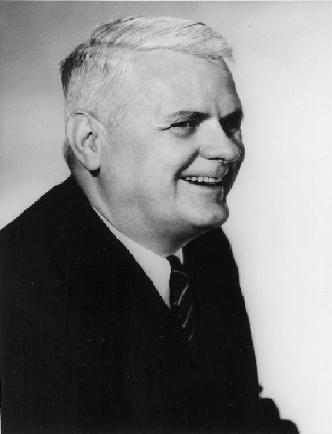
\includegraphics[scale=.50]{church}
    \end{column}
    \begin{column}{.49\textwidth}
      \itemize{
      \item Alonzo Church - 1936
      \item $\lambda$ Calculus
       \footnote{\href{https://www.ics.uci.edu/~lopes/teaching/inf212W12/readings/church.pdf}
         {An Unsolvable Problem of Elementary Number Theory}}
      }

    \end{column}
  \end{columns}
}

\frame{
  \frametitle{Origins of Clojure - McCarthy}
  \begin{columns}
    \begin{column}{.49\textwidth}
      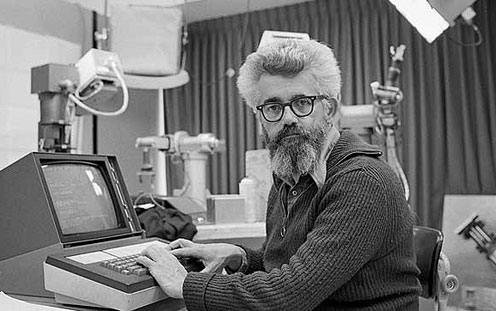
\includegraphics[width=\textwidth,height=\textheight,keepaspectratio=true]{john-mccarthy}
    \end{column}
    \begin{column}{.49\textwidth}
      % \vspace {4 cm}
      \itemize{
      \item John McCarthy - 1958
      \item
        OriginalPaper - 1960
        \footnote{\href{http://www-formal.stanford.edu/jmc/recursive.html}{Original Paper}}
      \item 
        Influenced by Church \& IPL 
        \footnote{\href{https://en.wikipedia.org/wiki/Information_Processing_Language}{
            IPL Overview}}
        \vspace {4 cm}
      }
    \end{column}
  \end{columns}
}

\frame{
  \frametitle{Origins of Clojure - Steve Russell - 1958}
  \begin {columns}
    \begin{column}{.49\textwidth}
      \begin{itemize}
      \item[] 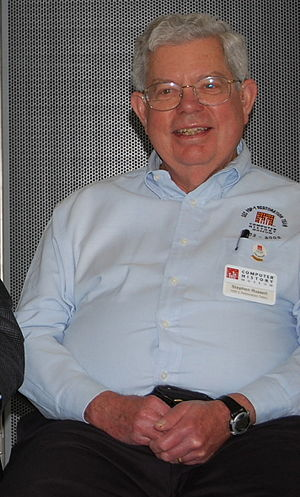
\includegraphics[scale=1.25]{steve-russell}
      \item[] First Lisp interpreter
      \end{itemize}
    \end{column}
    \begin{column}{.49\textwidth}
      \begin{itemize}
      \item[]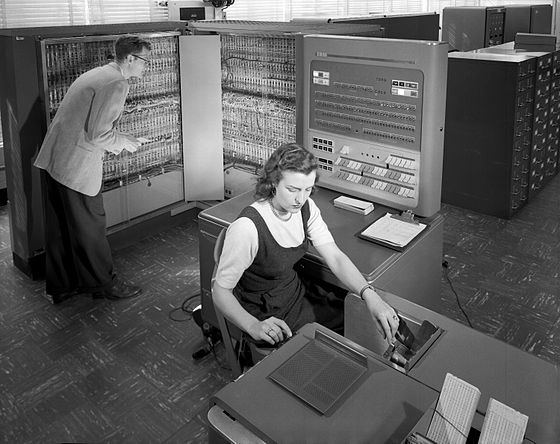
\includegraphics[scale=1.35]{ibm-704}
      \item[]IBM-704
      \end{itemize}
    \end{column}
  \end{columns}
}

\frame{
  \frametitle{Notable Attributes of the Original Lisp}
  \begin{itemize}
  \item Conditionals
  \item A function type
  \item Recursion
  \item Variables as pointers
  \item Garbage Collection
  \end{itemize}
}

\frame{
  \frametitle{Many Lisp Implementations}
  % 
  % TODO add more?
  % 
  \begin{itemize}
  \item Maclisp - Late 1960s \footnote{MIT, not Apple}
  \item Scheme - 1970s (Guile, Racket, Chicken) 
  \item Emacs LISP - 1976
  \item Common LISP - 1984 (CLISP, CMUCL, SBCL, ABCL, MKCL)
  \item AutoLISP - 1986
  \item Apple Dylan - 1992
  \item Clojure - 2007
  \item Arc - 2008
  \end{itemize}
}

\frame{
  \frametitle{Origins of Clojure - Communicating Sequential Processes (CSP) - 1977}
  \begin {columns}
    \begin{column}{.49\textwidth}
      \begin{itemize}
      \item[] 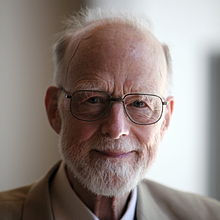
\includegraphics[scale=.75]{Tony_Hoare}
      \item[] Tony Hoare
      \end{itemize}
    \end{column}
    \begin{column}{.49\textwidth}
      \begin{itemize}
        \item[] Foundation of core.async
      \end{itemize}
    \end{column}
  \end{columns}
}


\frame{
  \frametitle{Origin of Clojure - Persistent Data Structures - 1989}
  \begin {columns}
    \begin{column}{.49\textwidth}
      \begin{itemize}
      \item James R. Drisco
      \item Neil Sarna
      \item Daniel D. Sleat
      \item Robert E. Tawa
      \end{itemize}
    \end{column}
    \begin{column}{.49\textwidth}
      \begin{itemize}
        
      \item \href{http://www.cs.cmu.edu/~sleator/papers/another-persistence.pdf}{\color{blue}{
            Making Data Structures Persistent}}
      \end{itemize}
    \end{column}
  \end{columns}
}


\frame{
  \frametitle{Origins of Clojure - Bagwell - 2001}
  \begin {columns}
    \begin{column}{.49\textwidth}
      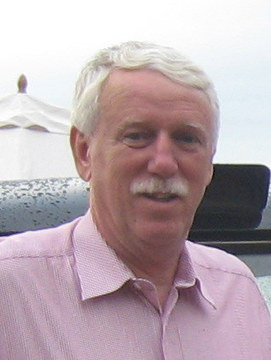
\includegraphics[scale=1]{phil-bagwell}
      \vspace {.25 cm}
    \end{column}
    \begin{column}{.49\textwidth}
      \begin{itemize}
      \item \href
        {https://infoscience.epfl.ch/record/64398/files/idealhashtrees.pdf}{\color{blue}{
            Ideal Hash Trees}}
      \item Hash Array Mapped Trie (HAMT)
      \end{itemize}

    \end{column}
  \end{columns}
  Phil Bagwell
}

\frame{
  \frametitle{Origins of Clojure - Hash Array Mapped Trie}
  \center { $O(log_{32} n)$ Effectively Constant Time}
  %\vspace {.25 cm}
  \center{
    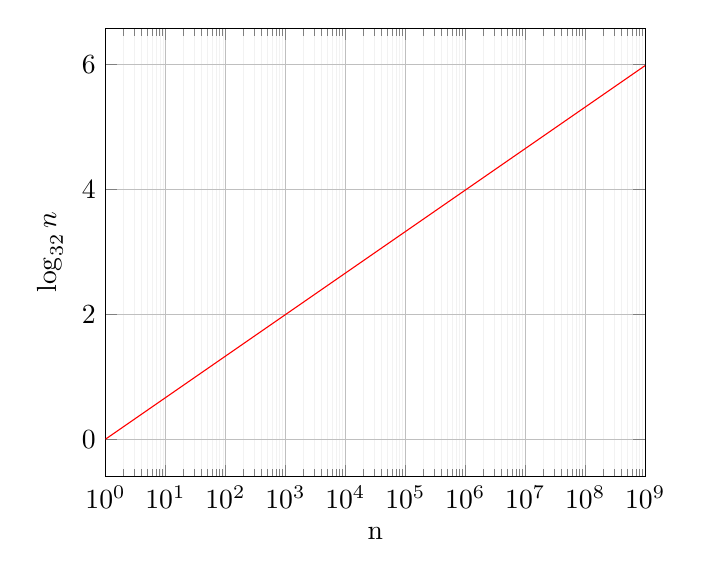
\begin{tikzpicture}
      \begin{semilogxaxis}[
        grid=both,
        grid style={line width=.1pt, draw=gray!10},
        major grid style={line width=.2pt,draw=gray!50},
        xmin=1,
        xmax=1000000000,
        domain=1:1000000000,
        ylabel=$\log_{32} n$,
        xlabel=n]
        % 
        % recall that log32(x) = log10(x) / log10(32)
        % 
        \addplot[
        red,
        ]
        {log10(x) / log10(32)};
      \end{semilogxaxis}
    \end{tikzpicture}
  }
  %\vspace {.25 cm}
  %\center{ \tiny{Effectively Constant Time} }
}


\frame{
  \frametitle{Origins of Clojure - Hickey 2007}
  \center{
    
\includegraphics[scale=.45]{rhickey}
  }
  Rich Hickey
}

\frame{
  \frametitle{Yet Another Lisp?}
  \begin{itemize}
    % \pause
  \item Immutability is the Default 
    % \pause
  \item Persistent Collections
    % \pause
  \item Unified Sequences (Lists, Maps, Vectors, Sets)
    % \pause
  \item Concurrency Support
    % \pause
  \item Designed to rely on (and embrace) a host platform
    % \pause
  \item JVM
    % \pause
  \item Javascipt (Browser and Node)
    % \pause
  \item CLR (.NET)

    % 
    % Mention clojurescript has laid the ground-work of clojure-in-clojure
    % 
    % \item Embraces the host platform (Predominantly the JVM)
    %   \pause
    % \item Clojurescript brings Clojure to the browser/node environment
    %   \pause
  \end{itemize}
}

% TODO - Add Stuart Halloway attribution here...
\frame{
  \frametitle{Clojure's Worldview}
  \begin{itemize}
  \item Data Centric 
  \item Data should not be hidden behind objects
  \item Mutable state makes concurrency, and most other things hard
  \item VMs not Operating Systems
  \item Fight with the army we have (parasitic language - rely on a
    host env)
  \item Disciplined Evolution
  \item There is wisdom in history
  \end{itemize}
}

% Consider borrowing some ideas from this: 
%https://www.reddit.com/r/Clojure/comments/mcuq3s/clojure_in_a_nutshell_by_james_trunk/?utm_source=share&utm_medium=web2x&context=3

\frame{
  \frametitle {Obligatory Quote}
  \say{Some programming languages have been created primarily to demonstrate
    a particular nugget of academia or to explore certain theories of
    computation. Clojure is not one of these. Rich Hickey has said on
    numerous occasions that Clojure has value to the degree that it lets
    you build interesting and useful applications.}
  \rightline{{\rm --- The Joy of Clojure}}
}

\frame{
  \frametitle {Obligatory Quote}
  \say {By relieving the brain of all unnecessary work, a good notation sets
    it free to concentrate on more advanced problems.}
  \rightline{{\rm --- Alfred North Whitehead}}
}

% TODO - revaluate if this table is helpful for an introduction.
% Update - I don't think it is. Should probably Remove for now...
% 
\begin{frame}
  \frametitle{Core Clojure Syntax}
  \begin{tabularx}{\textwidth}{ |X|X|X| }
    \hline
    \emph{Function invocation} & (fn-name fn-arg...)  &  (foo 1 2 3) \\ 
    \hline
    \emph{Keyword} & :key  & :foo \\ 
    \hline
    \emph{Map} &    \{\}  & \{:a 1 :b 2 :c 3\} \\ 
    \hline
    \emph{Set} &    \#\{\} & \#\{1 2 3\} \\ 
    \hline
    \emph{Vector} & []  & [1 2 3] \\
    \hline
    \emph{List} & '() & '(1 2 3) \\
    \hline
    \emph{Regex} & \#"" & \#"*.clj" \\    
    \hline
  \end{tabularx}

  \vspace{.5cm}
  Syntax is essentially (fn/macro-name arg1 arg2 ...) where arguments can
  be functions, constants, or data literals. 
\end{frame}

\begin{frame}[fragile]
  \frametitle{Core Clojure Syntax}
  \center{
    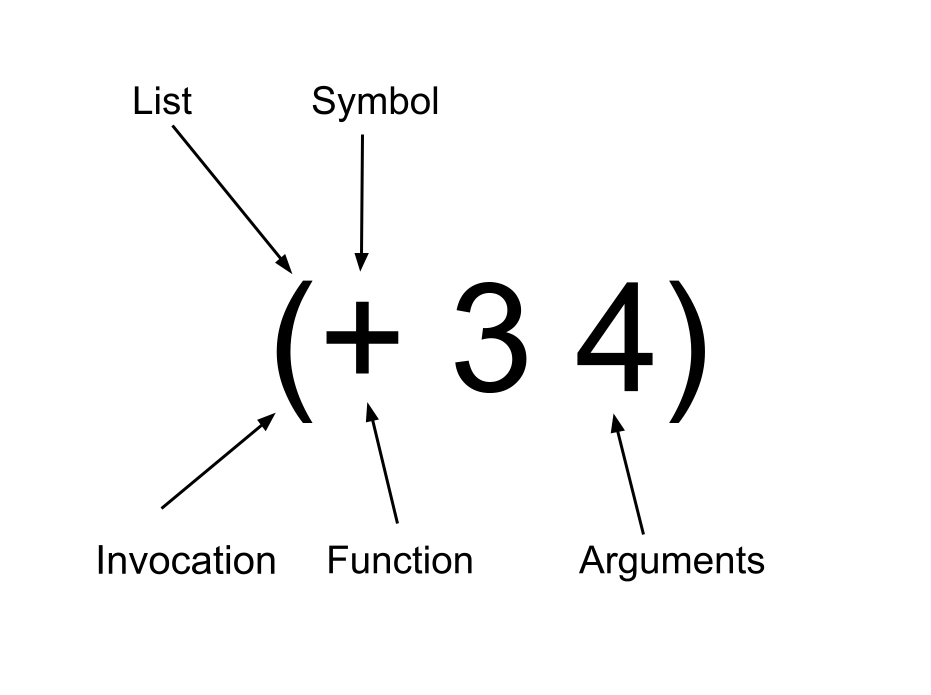
\includegraphics[scale=.25]{clojure-form}
  }
\end{frame}

\begin{frame}[fragile]
  \frametitle{Core Clojure Syntax - Data Literals}
  \begin{minted}[fontsize=\small]{clojure}
;;keyword
:jenny

;;list
'(1 2 3 4 5)

;;vector
[8 6 7 5 309]                                  

;;map
{:first-name "Tommy" :last-name "Tutone"}      

;;set
#{19 81}                                       

;;regex
#"^(.+)@(.+)$"
\end{minted}  
\end{frame}

\begin{frame}[fragile]
  \frametitle{Core Clojure Syntax - Data Literals}
  \begin{minted}[fontsize=\tiny]{java}
package cafebabe.prototypes;

public class Empty {
}
  \end{minted}
  \begin{minted}[fontsize=\tiny]{clojure}
;;composite structure

{:header        {:magic 3405691582 :major-version 0 :minor-version 52}
 :constant-pool [{:constant-type :c-method-ref :class-index 3 :name-and-type-index 10}
                 {:constant-type :c-class :name-index 11}
                 {:constant-type :c-class :name-index 12}
                 {:constant-type :c-utf8 :str "<init>"}
                 {:constant-type :c-utf8 :str "()V"}
                 {:constant-type :c-utf8 :str "Code"}
                 {:constant-type :c-utf8 :str "LineNumberTable"}
                 {:constant-type :c-utf8 :str "SourceFile"}
                 {:constant-type :c-utf8 :str "Empty.java"}
                 {:constant-type :c-name-and-type :descriptor-index 4 :name-index 5}
                 {:constant-type :c-utf8 :str "cafebabe/prototypes/Empty"}
                 {:constant-type :c-utf8 :str "java/lang/Object"}]
 :access-flags  33
 :this-class    2
 :super-class   3
 :interfaces    []
 :fields        []
 :methods       [{:access-flags     1
                  :name-index       4
                  :descriptor-index 5
                  :attributes       [{:attribute-name-index 6
                                      :info                 [0 1 0 1 0 0 0 5 183 0 1 177 0 0
                                                             0 1 0 7 0 0 0 6 0 1 0 0 0 6]}]}]
 :attributes    [{:attribute-name-index 8 :info [0 9]}]}

\end{minted}  
\end{frame}

%% \begin{frame}
%%   \frametitle{Limited Syntax Budget}
%%   \begin{itemize}
%%   \item Data Literals 
%%   \item Reader Macros
%%   \item Destructuring
%%   \end{itemize}
%% \end{frame}

%% \begin{frame}
%%   \frametitle{Syntax Sugar (Reader Macros)}
%%   % 
%%   % put table here...
%%   % 
%% \end{frame}




\begin{frame}[fragile]
  \frametitle{Functions}
  Typical function definition:
  \begin{minted}[fontsize=\normalsize,escapeinside=||]{clojure}
    (defn foo 
      "optional multiline doc comment"
      {:optional :metadata-map} 
      [arg1 arg2]
      (...implementation...))
  \end{minted}

  \vspace{1 cm}

%% [autogobble,fontfamily=myfont,escapeinside=||}{c}

  This is an anonymous function (sum of its args):
  \begin{minted}[fontsize=\normalsize]{clojure}
    (fn [a b] (+ a b))   
  \end{minted}
  \vspace{1 cm}

  An abbreviated equivalent:
  \begin{minted}[fontsize=\normalsize]{clojure}
    #(+ %1 %2)
  \end{minted}
\end{frame}

\begin{frame}[fragile]
  \frametitle{Multi-arity Functions}
  \begin{minted}[fontsize=\normalsize]{clojure}
  
  (defn make-set 
    ([x]   #{x}) 
    ([x y] #{x y}))

  (make-set 1)
  => #{1}

  (make-set 1 2)
  => #{1 2}
  
  (make-set 1 2 3)
  => ArityException Wrong number of args passed...
\end{minted}
\end{frame}

\begin{frame}[fragile]
  \frametitle{Function Pre/Post Conditions}
  \begin{minted}[fontsize=\normalsize]{clojure}
(defn constrained-fn [f x]
  {:pre  [(pos? x)]
   :post [(= % (* 2 x))]}
  (f x))

(constrained-fn #(* 2 %) 2)
=> 4
(constrained-fn #(float (* 2 %)) 2)
=> 4.0
(constrained-fn #(* 3 %) 2)
=> java.lang.Exception: Assert failed: (= % (* 2 x))
  \end{minted}
\end{frame}

\begin{frame}[fragile]
  \frametitle{Functions}
  \begin{minted}[fontsize=\normalsize]{clojure}
    ;; Keywords are functions which take a map as an
    ;; argument
    (:a {:a 1 :b 2 :c 3})
    => :1

    (:d {:a 1 :b 2 :c 3})
    => nil

    ;;Sets are functions of their elements that return the 
    ;;matched element or nil: 
    (#{:a :b :c :d} :c)
    => :c

    (#{:a :b :c :d} :e)
    => nil

  \end{minted}
\end{frame}

\begin{frame}[fragile]
  \frametitle{Functions}
  \begin{minted}[fontsize=\normalsize]{clojure}
    ;; Vectors are functions which take an integer index and return the element at
    ;; that position.
    ([1 2 3] 0)
    => 1

    ([1 2 3] 2)
    => 3

    ;;Maps are functions which accept a argument to be used as a key to find an item
    ;;in the map. Nil is returned if the key does not exist in the map.
    ({:a 1 :b 2 :c 3} :c)
    => 3

    ({:a 1 :b 2} :e)
    => nil

  \end{minted}
\end{frame}


\begin{frame}
  \frametitle{Multimethods}
\end{frame}

\begin{frame}[fragile]
  \frametitle{Control Flow Primitives}
  \begin{minted}[linenos=false,fontsize=\normalsize]{clojure}
    (+ 1 2 3 4)
    #"some regex"

  \end{minted}
\end{frame}

%%\begin{frame}
%
% Review JOC on this subject.
%
%%   \frametitle{Truthiness}
%% \end{frame}


\begin{frame}
  \frametitle{Sequences}
  \itemize {
  \item Referred to as Seqs (pronouced seeks)
  \item Unified interface for maps, lists, vectors, and sets  
  }
\end{frame}

\begin{frame}
  \frametitle{Map Binding Forms}
  % Look here from some inspiration http://stuartsierra.com/2010/01/15/keyword-arguments-in-clojure
\end{frame}

%% \begin{frame}
%%   \frametitle{Lazy-Seq TODO}
%% \end{frame}

%% \begin{frame}
%%   \frametitle{vars and refs}
%%  
%%\end{frame}

\begin{frame}
  \frametitle{namespaces}
  \itemize{
  \item clojure.lang.Namespace
  \item current accessible via nsy
  }  
\end{frame}

\begin{frame}[fragile]
  \frametitle{Host Interop}
  \begin{minted}[fontsize=\small]{clojure}
;; instance method invocation
=> (.toUpperCase "fred")
"FRED"

;; classnames yield Class values
=> (.getName String)
"java.lang.String"

;; constructor syntax 'Classname.'
(def p (java.awt.Point. 1 2))

;; field accessor
=> (.-x p)
1

;; static method
=> (System/getProperty "java.vm.version")
"25.151-b12"

;; static field
=> Math/PI
3.141592653589793
  \end{minted}
%% Mention bean?
\end{frame}

\begin{frame}
  \frametitle{Metadata}

\end{frame}

\begin{frame}
  \frametitle{REPL}
  % 
  % Useful repl stuff here...inspect-tree inspect-table javadoc doc
  % source
  % Must mention pst fn - invaluable!

\end{frame}

\begin{frame}
  \frametitle{REPL Debugging}
% 
% pst - very useful!
%

\end{frame}

\begin{frame}
  \frametitle{Code Samples} 
  \inputminted{clojure}{src/xml-parse.clj}
\end{frame}  

\begin{frame}
  \frametitle{Clojure}
  \center{
    
\includegraphics[scale=.20]{clojure-cave}
  }

  % Look at wikimedia commons for fair use pictures

\end{frame}

%https://clojure.org/api/cheatsheet

\frame {
  \frametitle{Resources}
  \begin{itemize}

  \item \href {https://www.clojure-toolbox.com/}
    {\color {blue}{Curated List of Libraries}}

  \item \href {https://clojure.org/api/cheatsheet}
    {\color {blue}{Cheatsheet}}

  \item \href {https://clojure.org/about/history}
    {\color {blue}{History of Clojure}}

 \item \href {https://www.braveclojure.com/}
    {\color {blue}{CLOJURE for the BRAVE and TRUE}}
  
  \item \href{https://github.com/edn-format/edn}
    {\color {blue}{Extensible Data Notation (EDN)}}

  \item \href{https://reagent-project.github.io/}
       {\color {blue}{Reagent (clojurescript + React = greatness)}}

  \item \href{https://github.com/tstout/examples/blob/master/clojure/slides/clojure-basics.tex}
       {\color {blue}{Code for this document}}

  \end{itemize}
  }

% 
% Let over lambda example...can simplify with #()
% 
% (defn db-layer [db-connection]
% (let [db-operations {:save (fn [obj] (save db-connection obj))
% :delete (fn [obj] (delete db-connection obj))
% :query (fn [query] (query db-connection query))}]
% (fn [operation & params]
% (-> (db-operations operation) (apply params)))))
\end{document}
